\documentclass[border=5pt]{standalone}
\usepackage{tikz}
\usepackage{pgfplots}
\pgfplotsset{compat=1.18}

\begin{document}
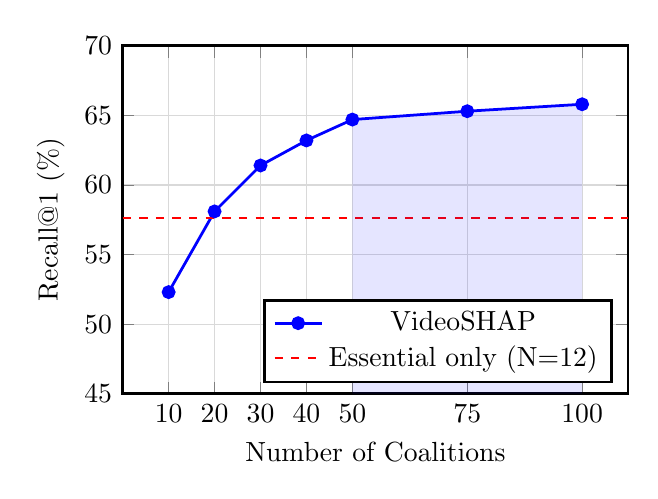
\begin{tikzpicture}
\begin{axis}[
    width=8cm,
    height=6cm,
    xlabel={Number of Coalitions},
    ylabel={Recall@1 (\%)},
    xmin=0, xmax=110,
    ymin=45, ymax=70,
    xtick={10,20,30,40,50,75,100},
    ytick={45,50,55,60,65,70},
    legend pos=south east,
    grid=both,
    grid style={gray!30},
    line width=1pt,
]

% Main performance curve
\addplot[
    color=blue,
    mark=*,
    mark size=2pt,
] coordinates {
    (10, 52.3)
    (20, 58.1)
    (30, 61.4)
    (40, 63.2)
    (50, 64.7)
    (75, 65.3)
    (100, 65.8)
};
\addlegendentry{VideoSHAP}

% Essential coalitions baseline (dashed line)
\addplot[
    color=red,
    dashed,
    thick,
] coordinates {
    (0, 57.6)
    (110, 57.6)
};
\addlegendentry{Essential only (N=12)}

% Shaded region for diminishing returns
\addplot[
    fill=blue,
    fill opacity=0.1,
    draw=none,
] coordinates {
    (50, 45)
    (50, 64.7)
    (100, 65.8)
    (100, 45)
} -- cycle;

\end{axis}
\end{tikzpicture}
\end{document}
